% !TEX root = main.tex
\section{Implementation of a Dataflow Library in QL for SSA-dIMP}
In this section, we describe an implementation of the algorithm schema described in the
last section.
The implementation is written in QL.
As part of the project, we implemented a library and a database schema for SSA-dIMP.
On top of that, the dataflow algorithm is implemented.

The implementation itself is very easy, but the structure follows the
dataflow library used for Java.
It is useful, because it demonstrates how to bridge the gap between
the theoretical description of the algorithm with the soundness proof
as in \autoref{sec:df-theory} and the actual implementation of dataflow
in QL for languages like Java.
However, all the features that complicate the dataflow library for Java have been 
omitted.
The most complicated feature is that the Java dataflow library supports tracking 
flow through fields, i.e.\ if a variable that received data from a source 
is assigned to a field in an object, and a sink later reads from that field,
dataflow is detected.
Furthermore, the Java dataflow library is an interprocedural analysis.
Thus, the implementation has to be done very carefully to exhibit good
performance on large projects.

\subsection{The Database Schema}
The database contains a representation the abstract syntax tree (AST) of the program.
Its schema is given in full in the \hyperref[lst:dbschema]{appendix}.
For each arithmetic expression, its unique ID, its kind
(i.e.\ integer literal, addition, multiplication, \ldots) 
and the ID of the type of the expression are saved.
Furthermore, another table contains the parent-child relation for arithmetic 
expressions --- every tuple there contains the ID of an expression parent 
(either an arithmetic expression, a Boolean expression or a statement),
the ID of the child arithmetic expression and the index.
For example the addition $a_0 + a_1$ has as first child the ID of the expression 
$a_0$, and as second child the ID of the expressions $a_1$.
The order of these is an implementation detail of the database schema in combination
with the extractor (that writes the database) and the standard library 
(that is built on top of the database schema).

A similar database layout is employed for statements and Boolean expressions.
Expressions like literals have another relation that tracks the actual value of the
literal, variable reads have a relation that tracks the variable that is read,
variable assignments have a relation that tracks the variable that is assigned to, etc.

The database schema is quite close how a compiler would model an AST for SSA-dIMP.
It is certainly inspired by the QL database schema for Java.
There is one crucial difference though --- in SSA-dIMP the AST is already in SSA form,
and we assume that sets $\Gamma, \Delta$ exist to prove that.
Programs in Java are not in SSA form.
Thus, as part of the QL library for Java, there exists an SSA construction algorithm
that synthesizes an SSA form.
As this is computed on the fly, it is not represented in the database schema.

Essentially, this makes the implementation of the library for SSA-dIMP easier,
as we don't have to deal with the SSA construction.
Constructing the SSA form of a program is a well-researched problem in compiler
construction, so we feel confident that assuming the existence of an SSA form 
of the program does not lower the value of this project.

\subsection{The Standard Library}
The standard library for SSA-dIMP is implemented in the file \hyperref[lst:library]{library.qll}.
It offers an object-oriented interface on top of the relational
database schema.
This interface is inspired by the corresponding library for Java.

The library offers interfaces for arithmetic expressions, and each kind of expression
has a sub-class available in the standard library.
As the QL language requires toString predicates on all classes,
the standard library also provides pretty-printing for the entire AST.

Furthermore, for example the class representing a Variable offers access to the
reads of that variable (phi nodes and variable access expressions), as well
as access to the statements that assign to this variable.
Also, the parent-child relation is exposed, and used to implement named helper predicates.
For example, for an if statement, the child branches are exposed as \texttt{getThenBranch()}
and \texttt{getElseBranch()}.
This hides the implementation detail that the then branch is the first child of the
if statement, and the else branch the second.

\subsection{The Dataflow Algorithm}
As the algorithm in \autoref{sec:df-theory} computes a type for all expressions and statements in the program,
it implicitly runs on the AST.
The algorithm in practice is given in \hyperref[lst:dataflow]{dataflow.qll}.

\subsubsection*{Step 1 --- The Dataflow Graph}
The algorithm given here (unlike the DF rules) does not run on the entire AST of the program,
but on a different graph, the \emph{dataflow graph}.
It is a datastructure that makes it easy to compute the typing derivation needed to
detect dataflow.
The node set of the dataflow graph is a subset of the node set of the AST.

The dataflow graph keeps track of which expressions and statements potentially get data from a source.
The node set of the dataflow graph contains all AST nodes of the following form:
\begin{itemize}
    \item all expressions of kind variable access and source
    \item statements of kinds assign and sink
    \item all $\varphi$-nodes
\end{itemize}

All of these nodes then get tagged in step 2 with a label.
For the expressions, this directly corresponds to the type in the refined type system
as presented in~\autoref{sec:df-theory}.
For assign statements and $\varphi$-nodes, this label corresponds to the type of 
the variable that is defined, and for sinks the label corresponds to the type
of the expression that is passed to the sink.

We can restrict the node set to these expression kinds, as all other expression kinds
are always tagged with $\lclean$.
The only relevant statements for dataflow are assign and sink, as all DF rules for the 
other statements just pass through labels, but don't define new labels.
Thus, the node set contains  exactly the relevant elements of the AST that are involved in determining
if a program has dataflow or not.

Building the dataflow graph is done by defining the \texttt{flowStep} relation on the node set.
It contains the tuple $(\textit{node1}, \textit{node2})$ if the label of \textit{node2} is directly affected
by the label of \textit{node1}.
Thus, the edges of the dataflow graph indicate along which paths dataflow tracking marker propagate
through the program.

For example, if an expression node has type $\ltracked$,
all downstream expression nodes on a path from the first expression node 
have type either $\ltracked$ or $\lunknown$ (and not $\lclean$).
We combine this propagation information with the location of the sinks and sources 
to detect potential dataflow.

The dataflow graph contains the following edges:
\begin{itemize}
    \item From the expression on the right-hand side of an assign statement 
    to the statement node of the assignment
    \item From the expression that is passed into a sink statement to the statement node
    of the sink
    \item From a $\varphi$-node defining a variable to all expression nodes reading 
    that variable, and to all $\varphi$-nodes having that variable as input
    \item From an assign statement defining a variable to all expression nodes reading 
    that variable, and to all $\varphi$-nodes having that variable as input
\end{itemize}

By looking at the typing rule for statements, we see that only assign and sink statements
use the tracking marker assigned to the arithmetic expression used in that statement.
Thus, those are the nodes that receive incoming edges from their operands.

The other cases in \texttt{flowStep} deal with variable definitions.
The intention is that there is an edge from every variable definition to all of its uses,
regardless of how the definition and use look like in the AST.

There are no incoming edges for source expressions, as the result of a source expression
is always tainted.

We now show the dataflow graph for the example program (\autoref{fig:ssa-dimp-example}).
Node types (expression, $\varphi$ or statement) are not indicated, but are obvious from context.
Furthermore, the place of the variable accesses in the AST is indicated by giving the 
line numbers (referring to the SSA-dIMP program).
As every node in the dataflow graph is also a node in the AST, all the variable accesses
of one variable are different nodes in the dataflow graph.

\begin{figure}[h]
    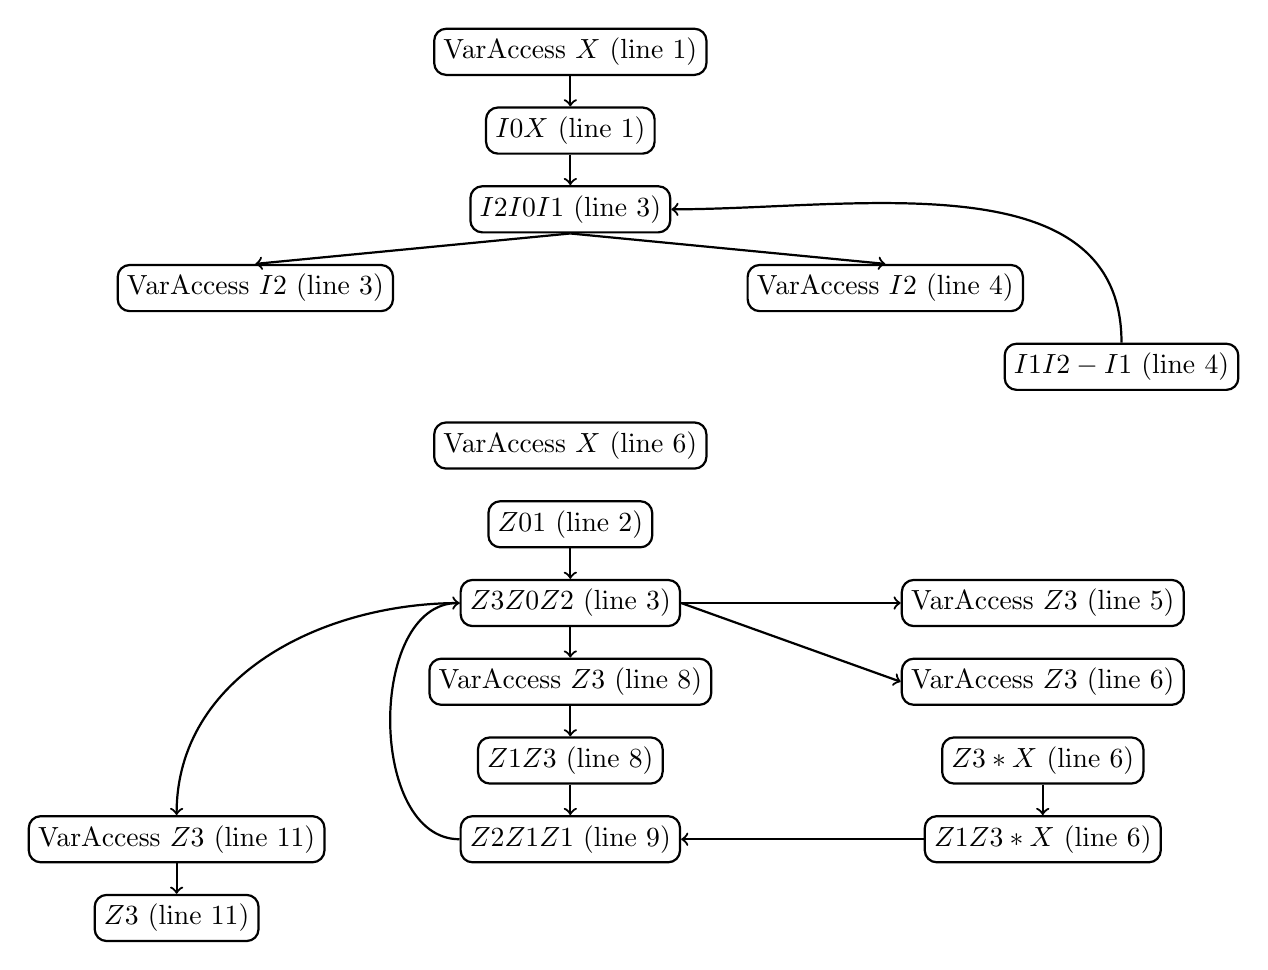
\begin{tikzpicture}[roundnode/.style={rectangle,rounded corners=1ex,draw=black!100,thick},->,thick]
        \node[roundnode] (storez0) at(0, 1) {$\storecmd{Z0}{1}$ (line 2)};
        \node[roundnode] (phiz3) at (0, 0) {$\phistore{Z3}{Z0}{Z2}$ (line 3)};
        \node[roundnode] (varaccessbool) at (6, 0) {VarAccess $Z3$ (line 5)};
        \node[roundnode] (multvaraccess) at (6, -1) {VarAccess $Z3$ (line 6)};
        \node[roundnode] (source) at (6, -2) {$\source{Z3 * X}$ (line 6)};
        \node[roundnode] (storemult) at (6, -3) {$\storecmd{Z1}{\source{Z3 * X}}$ (line 6)};
        \node[roundnode] (multvaraccess2) at (0, 2) {VarAccess $X$ (line 6)};
        \node[roundnode] (varaccessz4) at (0, -1) {VarAccess $Z3$ (line 8)};
        \node[roundnode] (storez1) at (0, -2) {$\storecmd{Z1}{Z3}$ (line 8)};
        \node[roundnode] (phiz2) at (0, -3) {$\phistore{Z2}{Z1}{Z1}$ (line 9)};
        \node[roundnode] (varaccessz42) at (-5, -3) {VarAccess $Z3$ (line 11)};
        \node[roundnode] (sink) at (-5, -4) {$\sink{Z3}$ (line 11)};
        \draw (storez0.south) -- (phiz3.north);
        \draw (phiz3.east) -- (varaccessbool.west);
        \draw (phiz3.east) -- (multvaraccess.west);
        \draw (storemult.west) -- (phiz2.east);
        \draw (phiz3.south) -- (varaccessz4.north);
        \draw (varaccessz4.south) -- (storez1.north);
        \draw (storez1.south) -- (phiz2.north);
        \draw (phiz2.west) to [out=180,in=180] (phiz3.west);
        \draw (phiz3.west) to [out=180,in=90] (varaccessz42.north);
        \draw (varaccessz42.south) -- (sink.north);
        \draw (source.south) -- (storemult.north);
        \node[roundnode] (ivarx) at (0, 7) {VarAccess $X$ (line 1)};
        \node[roundnode] (i0getsx) at (0, 6) {$\storecmd{I0}{X}$ (line 1)};
        \node[roundnode] (phii2) at (0, 5) {$\phistore{I2}{I0}{I1}$ (line 3)};
        \node[roundnode] (readi21) at (-4, 4) {VarAccess $I2$ (line 3)};
        \node[roundnode] (readi22) at (4, 4) {VarAccess $I2$ (line 4)};
        \node[roundnode] (writei1) at (7, 3) {$\storecmd{I1}{I2 - I1}$ (line 4)};
        \draw (ivarx.south) -- (i0getsx.north);
        \draw (i0getsx.south) -- (phii2.north);
        \draw (phii2.south) -- (readi21.north);
        \draw (phii2.south) -- (readi22.north);
        \draw (writei1.north) to [out=90,in=0] (phii2.east);
    \end{tikzpicture}
    
    \caption{The dataflow graph for the example program}
    \label{fig:df-graph}
\end{figure}

\subsubsection*{Step 2 --- Labeling Nodes}
\newcommand{\coloredset}[1]{{\color{red}$\{#1\}$}}
\newcommand{\setclean}{\coloredset{\labclean}}
\newcommand{\settracked}{\coloredset{\labtracked}}
\newcommand{\setboth}{\coloredset{\labclean, \labtracked}}
\newcommand{\clclean}{:\ {\color{red}$\lclean$}}
\newcommand{\cltracked}{:\ {\color{red}$\ltracked$}}
\newcommand{\clunknown}{:\ {\color{red}$\lunknown$}}

As second step, the algorithm computes a labelling of the nodes of the dataflow graph.
Possible labels are \labclean, \labtracked and \labunknown.
This labelling can be used to easily determine if a program is safe to execute or not.
Furthermore, this labelling can be used to construct a typing derivation (by the DF-rules)
of the program.

As QL is built to be a query language, programming in QL is significantly different
from imperative general-purpose programming languages.
In particular, it doesn't have the concept of mutable state.
In an imperative language, implementing a dataflow algorithm would most
likely involve associating a label with each node that gets updated as the 
algorithm iterates.
A work list would keep track of nodes that need to be visited.

In QL, both is not possible.
Instead, the helper predicate \texttt{nodeLabelCand} computes a \emph{set} of
labels for each node.
Each label of a node belongs to one or more execution flows of the program 
that would result in that label being assigned.

Each source is marked with $\{\labtracked\}$, as in every program execution,
a source produce in a tracked value.
Furthermore, all nodes in the dataflow graph without
incoming edges that are not sources are marked with $\{\labclean\}$.
Nodes without incoming edges (that are not sources) represent either variable reads 
from variables defined in the initial store (these are clean by assumption), or 
assignments that read an expression that is clean by the DF rules, for example
a store of the result of a multiplication or addition.

Remember that in the dataflow graph, an edge from \textit{node1} to \textit{node2}
indicates that the label of \textit{node1} affects the label of \textit{node2}.
Thus, we propagate node labels along the edges of the dataflow path.
Every node receives all the labels of its predecessor(s), this includes
$\varphi$-nodes.

A $\varphi$-node indicates that two different control flows merge at the point
the $\varphi$-node is placed.
At analysis time, we do not know which branch(es) will be taken by the program,
so we approximate this behaviour by assuming that all branches will be taken at some point.
Thus, we propagate both incoming labels, even if they disagree.
This is different from the DF rules, that mandate that a single label is chosen
for a $\varphi$-node.

With these two recursive rules together we ensure that the label sets for each node
increase monotonically.
A least fixed point for that recursion is found when applying the recursive rules yields
no more nodes.

After all nodes are labelled with a set of labels, we still need to pick one annotated type
that correctly describes the node.
If a node is marked with $\{\labclean\}$, the type becomes $\lclean$,
and if a node is marked with $\{\labtracked\}$, the type becomes $\ltracked$.

If a node is marked with $\{\lclean, \ltracked\}$ it means that different
program execution paths result in a different tracked-markings for that node.
Thus, the node is assigned the type $\lunknown$.
This is in line with the side-condition of the rule \textsc{DF-$\varphi$}.

Assigning nodes an annotated type is implemented in the predicate \texttt{nodeLabel}.
The predicate computes the best-matching annotated type for each node using the candidate labels.
This happens after the propagation of labels (in \texttt{nodeLabelCand}) stabilizes.

With that information, the dataflow query can report all nodes of type sink.
If any of them has the type $\lunknown$ or $\ltracked$, then we know that the sink
is unsafe, because it (potentially) reads from a source.

To see how the candidate label computation works in practice, recall the dataflow graph
from~\autoref{fig:df-graph}.
We have included the annotated dataflow graph here at several stages of the algorithm:
\begin{enumerate}
    \item After the static initialization phase, but before the label propagation starts:
     ~\autoref{fig:label-graph-1}
    \item After the label propagation: ~\autoref{fig:label-graph-2}
    \item After the computation of the annotated types (i.e. the \texttt{nodeLabel} predicate):
     ~\autoref{fig:label-graph-3}
\end{enumerate}

\begin{figure}[h]
    \begin{tikzpicture}[roundnode/.style={rectangle,rounded corners=1ex,draw=black!100,thick},->,thick]
        \node[roundnode] (storez0) at(0, 1) {$\storecmd{Z0}{1}$ \setclean};
        \node[roundnode] (phiz3) at (0, 0) {$\phistore{Z3}{Z0}{Z2}$};
        \node[roundnode] (varaccessbool) at (6, 0) {VarAccess $Z3$};
        \node[roundnode] (multvaraccess) at (6, -1) {VarAccess $Z3$};
        \node[roundnode] (source) at (6, -2) {$\source{Z3 * X}$  \settracked};
        \node[roundnode] (storemult) at (6, -3) {$\storecmd{Z1}{\source{Z3 * X}}$};
        \node[roundnode] (multvaraccess2) at (0, 2) {VarAccess $X$  \setclean};
        \node[roundnode] (varaccessz4) at (0, -1) {VarAccess $Z3$ };
        \node[roundnode] (storez1) at (0, -2) {$\storecmd{Z1}{Z3}$ };
        \node[roundnode] (phiz2) at (0, -3) {$\phistore{Z2}{Z1}{Z1}$  };
        \node[roundnode] (varaccessz42) at (-5, -3) {VarAccess $Z3$ };
        \node[roundnode] (sink) at (-5, -4) {$\sink{Z3}$};
        \draw (storez0.south) -- (phiz3.north);
        \draw (phiz3.east) -- (varaccessbool.west);
        \draw (phiz3.east) -- (multvaraccess.west);
        \draw (storemult.west) -- (phiz2.east);
        \draw (phiz3.south) -- (varaccessz4.north);
        \draw (varaccessz4.south) -- (storez1.north);
        \draw (storez1.south) -- (phiz2.north);
        \draw (phiz2.west) to [out=180,in=180] (phiz3.west);
        \draw (phiz3.west) to [out=180,in=90] (varaccessz42.north);
        \draw (varaccessz42.south) -- (sink.north);
        \draw (source.south) -- (storemult.north);
        \node[roundnode] (ivarx) at (0, 7) {VarAccess $X$ \setclean};
        \node[roundnode] (i0getsx) at (0, 6) {$\storecmd{I0}{X}$};
        \node[roundnode] (phii2) at (0, 5) {$\phistore{I2}{I0}{I1}$};
        \node[roundnode] (readi21) at (-4, 4) {VarAccess $I2$ };
        \node[roundnode] (readi22) at (4, 4) {VarAccess $I2$ };
        \node[roundnode] (writei1) at (7, 3) {$\storecmd{I1}{I2 - I1}$  \setclean};
        \draw (ivarx.south) -- (i0getsx.north);
        \draw (i0getsx.south) -- (phii2.north);
        \draw (phii2.south) -- (readi21.north);
        \draw (phii2.south) -- (readi22.north);
        \draw (writei1.north) to [out=90,in=0] (phii2.east);
    \end{tikzpicture}
    
    \caption{The annotated dataflow graph after the initialization phase}
    \label{fig:label-graph-1}
\end{figure}

\begin{figure}[h]
    \begin{tikzpicture}[roundnode/.style={rectangle,rounded corners=1ex,draw=black!100,thick},->,thick]
        \node[roundnode] (storez0) at(-1, 1) {$\storecmd{Z0}{1}$ \setclean};
        \node[roundnode] (phiz3) at (-1, 0) {$\phistore{Z3}{Z0}{Z2}$ \setboth};
        \node[roundnode] (varaccessbool) at (6, 0) {VarAccess $Z3$ \setboth};
        \node[roundnode] (multvaraccess) at (6, -1) {VarAccess $Z3$ \setboth};
        \node[roundnode] (source) at (6, -2) {$\source{Z3 * X}$  \settracked};
        \node[roundnode] (storemult) at (6, -3) {$\storecmd{Z1}{\source{Z3 * X}}$  \settracked};
        \node[roundnode] (multvaraccess2) at (-1, 2) {VarAccess $X$  \setclean};
        \node[roundnode] (varaccessz4) at (-1, -1) {VarAccess $Z3$ \setboth};
        \node[roundnode] (storez1) at (-1, -2) {$\storecmd{Z1}{Z3}$  \setboth};
        \node[roundnode] (phiz2) at (-1, -3) {$\phistore{Z2}{Z1}{Z1}$  \setboth};
        \node[roundnode] (varaccessz42) at (-5, -4) {VarAccess $Z3$  \setboth};
        \node[roundnode] (sink) at (-5, -5) {$\sink{Z3}$ \setboth};
        \draw (storez0.south) -- (phiz3.north);
        \draw (phiz3.east) -- (varaccessbool.west);
        \draw (phiz3.east) -- (multvaraccess.west);
        \draw (storemult.west) -- (phiz2.east);
        \draw (phiz3.south) -- (varaccessz4.north);
        \draw (varaccessz4.south) -- (storez1.north);
        \draw (storez1.south) -- (phiz2.north);
        \draw (phiz2.west) to [out=180,in=180] (phiz3.west);
        \draw (phiz3.west) to [out=180,in=90] (varaccessz42.north);
        \draw (varaccessz42.south) -- (sink.north);
        \draw (source.south) -- (storemult.north);
        \node[roundnode] (ivarx) at (0, 7) {VarAccess $X$ \setclean};
        \node[roundnode] (i0getsx) at (0, 6) {$\storecmd{I0}{X}$ \setclean};
        \node[roundnode] (phii2) at (0, 5) {$\phistore{I2}{I0}{I1}$  \setclean};
        \node[roundnode] (readi21) at (-4, 4) {VarAccess $I2$ \setclean};
        \node[roundnode] (readi22) at (4, 4) {VarAccess $I2$ \setclean};
        \node[roundnode] (writei1) at (7, 3) {$\storecmd{I1}{I2 - I1}$  \setclean};
        \draw (ivarx.south) -- (i0getsx.north);
        \draw (i0getsx.south) -- (phii2.north);
        \draw (phii2.south) -- (readi21.north);
        \draw (phii2.south) -- (readi22.north);
        \draw (writei1.north) to [out=90,in=0] (phii2.east);
    \end{tikzpicture}
    
    \caption{The annotated dataflow after the label propagation}
    \label{fig:label-graph-2}
\end{figure}

\begin{figure}[h]
    \begin{tikzpicture}[roundnode/.style={rectangle,rounded corners=1ex,draw=black!100,thick},->,thick]
        \node[roundnode] (storez0) at(0, 1) {$\storecmd{Z0}{1}$ \clclean};
        \node[roundnode] (phiz3) at (0, 0) {$\phistore{Z3}{Z0}{Z2}$ \clunknown};
        \node[roundnode] (varaccessbool) at (6, 0) {VarAccess $Z3$ \clunknown};
        \node[roundnode] (multvaraccess) at (6, -1) {VarAccess $Z3$ \clunknown};
        \node[roundnode] (source) at (6, -2) {$\source{Z3 * X}$  \cltracked};
        \node[roundnode] (storemult) at (6, -3) {$\storecmd{Z1}{\source{Z3 * X}}$  \cltracked};
        \node[roundnode] (multvaraccess2) at (0, 2) {VarAccess $X$  \clclean};
        \node[roundnode] (varaccessz4) at (0, -1) {VarAccess $Z3$  \clunknown};
        \node[roundnode] (storez1) at (0, -2) {$\storecmd{Z1}{Z3}$   \clunknown};
        \node[roundnode] (phiz2) at (0, -3) {$\phistore{Z2}{Z1}{Z1}$   \clunknown};
        \node[roundnode] (varaccessz42) at (-5, -3) {VarAccess $Z3$   \clunknown};
        \node[roundnode] (sink) at (-5, -4) {$\sink{Z3}$  \clunknown};
        \draw (storez0.south) -- (phiz3.north);
        \draw (phiz3.east) -- (varaccessbool.west);
        \draw (phiz3.east) -- (multvaraccess.west);
        \draw (storemult.west) -- (phiz2.east);
        \draw (phiz3.south) -- (varaccessz4.north);
        \draw (varaccessz4.south) -- (storez1.north);
        \draw (storez1.south) -- (phiz2.north);
        \draw (phiz2.west) to [out=180,in=180] (phiz3.west);
        \draw (phiz3.west) to [out=180,in=90] (varaccessz42.north);
        \draw (varaccessz42.south) -- (sink.north);
        \draw (source.south) -- (storemult.north);
        \node[roundnode] (ivarx) at (0, 7) {VarAccess $X$ \clclean};
        \node[roundnode] (i0getsx) at (0, 6) {$\storecmd{I0}{X}$ \clclean};
        \node[roundnode] (phii2) at (0, 5) {$\phistore{I2}{I0}{I1}$  \clclean};
        \node[roundnode] (readi21) at (-4, 4) {VarAccess $I2$ \clclean};
        \node[roundnode] (readi22) at (4, 4) {VarAccess $I2$ \clclean};
        \node[roundnode] (writei1) at (7, 3) {$\storecmd{I1}{I2 - I1}$  \clclean};
        \draw (ivarx.south) -- (i0getsx.north);
        \draw (i0getsx.south) -- (phii2.north);
        \draw (phii2.south) -- (readi21.north);
        \draw (phii2.south) -- (readi22.north);
        \draw (writei1.north) to [out=90,in=0] (phii2.east);
    \end{tikzpicture}
    
    \caption{The annotated dataflow graph after selecting one annotated type for each node}
    \label{fig:label-graph-3}
\end{figure}

\subsubsection*{From QL to First-Order Predicate Logic}
In order to highlight how easy QL code translates into regular first-order predicate logic,
we give the direct translation of the predicates \texttt{nodeLabelCand} and \texttt{nodeLabel}
into first-order predicate logic.
These translations can be seen as the formalization of the textual algorithm description
from above.
They can also be put side-to-side to the QL source code, to see how predicate logic
syntax transfers to QL syntax.

The following helper predicates are used:
The predicate \texttt{sourceNode} contains only nodes that are of type expression,
where the expression is of kind source.
The predicate \texttt{flowStep} contains two nodes iff there is an edge in the dataflow 
graph (according to the rules described above).

\newcommand{\n}{\textit{node}}
\newcommand{\lab}{\textit{label}}
\newcommand{\labtwo}{\textit{label2}}
\newcommand{\prev}{\textit{prev}}
\begin{align*}
    \texttt{nodeLabelCand}(\n, \lab) :\iff &\texttt{sourceNode}(\n) \land \lab = \labtracked \\
    &\lor\\
    & \neg \texttt{sourceNode}(\n) \land (\\
    &\qquad\neg(\exists \prev: \texttt{flowStep}(\prev, \n)) \land \lab = \labclean\\
    &\qquad\lor\\
    &\qquad\exists \prev: (\texttt{flowStep}(\prev, \n) \land\\
    &\qquad \texttt{nodeLabelCand}(\n, \lab))\\
    &)
\end{align*}

\begin{align*}
    \texttt{nodeLabel}(\n, \lab) :\iff &\texttt{nodeLabelCand}(\n, \labclean) \land \\
    &\texttt{nodeLabelCand}(\n, \labtracked) \land \lab = \labunknown \\
    &\lor\\
    & \texttt{nodeLabelCand}(\n, \lab) \land\\
    &\neg (\exists \labtwo: \texttt{nodeLabelCand}(\n, \labtwo) \land \labtwo \neq \lab)\\
\end{align*}

The QL database engine then takes the predicates, orders them and comes up with 
a query plan that allows the computation of the set of tuples that are in both predicates.
In this example, there is a dependency of \texttt{nodeLabel} on \texttt{nodeLabelCand},
but not the other way round.
Thus, the predicate \texttt{nodeLabelCand} gets computed first, so that the evaluation
of \texttt{nodeLabel} can use the predicate \texttt{nodeLabelCand} in its computations.

%While the same logical formulation could probably also written in Prolog,
%at least on graphs with cycles Prolog would likely not terminate.

\subsubsection*{Recovering a Typing Derivation from a Labelled Dataflow Graph}
The information computed in step 2 is enough to detect unsafe sinks.
However, we can even go a step further and use the computed labels to build a
typing derivation for the whole program using the DF rules.
In case of programs that do not exhibit dataflow (as per the algorithm), this
typing derivation acts as an easily checkable certificate of the safety of the program.

Remember that the typing using the DF rules is a refinement of the typing provided 
by the SSA rules.
As we assume that all programs already have a typing derivation using the SSA rules,
we only need to supply the contents of the $\Delta$ and $\Gamma$ maps, as these 
type contexts keep track of the refined types.

The initial map $\Gamma$ is given by mapping all variables that are defined in 
the initial store to $\lclean$.

The $\Delta$ maps can be read of the type-annotated dataflow graph:
Only assign statements and invocations of the rule \textsc{DF-$\varphi$}
have non-empty $\Delta$ maps to begin with.
For assign statements, the assigned-to variable gets the type of the assign statement 
node in the dataflow graph.
For invocations of the \textsc{DF-$\varphi$} rule, we get the types of the 
variables defined in that list of $\varphi$-nodes by using the annotated
types in the dataflow graph of the individual $\varphi$-nodes.

These annotated types will satisfy the side-condition of the rule \textsc{DF-$\varphi$},
as we construct a solution to the constraints by basically hardcoding the join operator
of the poset.

Applied on example program as presented in~\autoref{fig:ssa-dimp-example} 
and using the annotated dataflow graph from~\autoref{fig:label-graph-3}, we 
can annotate all variable definitions with their type.
The types make up the contents of the $\Delta$ maps.
Given the types (and thus the $\Delta$ maps), the whole derivation tree can be easily written down.

\newcommand{\redltracked}{{\color{red}\ltracked}}
\newcommand{\redlclean}{{\color{red}\lclean}}
\newcommand{\redlunknown}{{\color{red}\lunknown}}

\begin{figure}[h]
    \begin{minted}[escapeinside=||,mathescape=false,linenos]{pascal}
        I0 |$:\redlclean$| := X;
        Z0 |$:\redlclean$| := 1;
        while [Z3 := |$\varphi$|(Z0, Z2) |$:\redlunknown$|, I2 |$:\redlclean$| := |$\varphi$|(I0, I1)]; I2 > 0 do
            I1 |$:\redlclean$| := I2 - 1;
            if Z3 < 100 then
                Z1 |$:\redltracked$| := source Z3 * X
            else
                Z1 |$:\redlunknown$| := Z3
            ;[Z2 |$:\redlunknown$| := |$\varphi$|(Z1, Z1)]
        ;
        sink Z3
    \end{minted}    
    \caption{The example programs annotated with types}
    \label{fig:delta-maps-example}
\end{figure}

\subsubsection*{On the Relation of the Algorithm to the DF Typing Rules}
As explained above, this algorithm runs already on SSA-dIMP, not dIMP.
Thus, we assume that the SSA construction already took place.
The transformation from dIMP to SSA-dIMP also (implicitly) takes care of the
concrete semantics of e.g.\ while and if statements --- the dataflow algorithm
only expects correctly placed $\varphi$-nodes,
and does not depend on the semantics of the individual statements.

If, for example, a repeat-until loop construct would be added to the language,
SSA-dIMP could be easily extended with that loop construct by adding a new statement 
kind to the database and implementing the library.
However, the dataflow algorithm itself would work without any changes, assuming that
the $\varphi$-node placement is correct.
This is very different from the algorithm schema with the DF rules that depends intimately on the 
typing schema, and this might be puzzling at first.
This apparent contradiction can be resolved by seeing that the DF typing 
rules serve two purposes --- first, they are a refinement of the SSA typing rules,
and second, they describe an approximation on where dataflow occurs.

As the dataflow algorithm as presented here assumes that the program is already in 
SSA form, it can do substantially less than what is described in the DF rules.
In particular, it only has to worry about the introduction of flow in expressions,
and the propagation of the tracked marking to variable stores and to sinks.
Thus, it can safely skip the entire part of the rules that deal with scoping.

%The tracked marker for variable reads is fully determined by the type context,
%which we do not explicitly compute.
%In the implicit formulation, a variable access gets the tracking marker of its definition,
%which is, because the program is in SSA form, unique.
%If the variable definition is an assign statement, this follows immediately from the
%\textsc{DF-Assign} rule - the variable is tagged with the marker of the expression.
%Thus, we have an edge from the expression node to that of the 
%If the variable is defined in a $\varphi$-node, we have compute the least upper bound of 
%both variables that make up the $\varphi$-node.
%This is implicit in the algorithm, as the $\varphi$-node will have an incoming edge if 
%at least one of the variables is marked with $\ltracked$ or $\lunknown$.
%However, in both cases, we have flow from a variable definition (either an assign
%statement or a $\varphi$-node) to a variable read (either a VarAccess expression, 
%or another $\varphi$-node).

\subsubsection*{Simplification of the Algorithm}
In practice, we can optimize the algorithm even more.
This is done by reducing the lattice and only keeping $\lclean$ and $\lunknown$.
Then, we do not need an explicit node label anymore, a predicate can now
keep track of all nodes that are marked with $\labunknown$ and that then later 
get assigned the type $\lunknown$.
These are the only relevant nodes for dataflow.
Furthermore, we can restrict ourselves to connected components of the dataflow graph
that start in a source node.
All other parts of the dataflow graph can be discarded, as they do not contribute 
to detecting dataflow.
In fact, nodes in this restricted dataflow graph are getting the type $\lunknown$ if there
exists a path from a source to the node.
Especially, this means a program is (potentially) dangerous if there exists a path
from a node of type source to a node of type sink.
This problem can be solved very efficiently.
The QL implementation can be found in the predicate \texttt{reaches},
that computes all reachable nodes from a sink.
If this predicate contains any sink nodes, the program is deemed unsafe.

This algorithm marks the same programs as unsafe as the previously proposed implementation,
but it does obviously not include the distinction between $\lunknown$ and $\ltracked$.
The theoretical groundwork as laid out in~\autoref{sec:df-theory} can be applied,
but using a two-point lattice with elements $\lunknown$ and $\lclean$ instead.
The soundness proof goes through essentially unchanged.
Thus, a typing derivation using the DF rules (with the simplified lattice) 
can be reconstructed, as explained above.

The example can also be adapted: In the example dataflow graph, one can easily
see that there is a path from the source to the sink, so that program is unsafe.

\subsection{The Query}
The query actually implementing the user-facing analysis is given in \hyperref[lst:query]{query.ql}.
It is very simple, it outputs a list of sinks if their annotated type is 
either $\ltracked$ or $\lunknown$.
If the list is empty, the program is safe and it is guaranteed by~\autoref{thm:soundness-df}
that the program has no dataflow.
If the list is not empty, no assertion about the program correctness can be given.

The difference between $\ltracked$ and $\lunknown$ is not reflected in the theoretical framework,
but it can be used to tailor the warnings given to the user.
If a sink is marked with $\ltracked$, that sink will abort the program, if it is ever
executed.
A sink that is marked with $\lunknown$ may abort the program, depending on control flow.
There is even the possibility that no control flow path exists at which the sink aborts 
the program.
Thus, the annotated types could be used to show sinks with $\ltracked$ with a higher
priority than sinks with $\lunknown$.

With a different operational semantics, this behaviour could be formalized, allowing us to
formally make the distinction in the output of the algorithm as well.
Currently, both $\ltracked$ and $\lunknown$ get mapped to POSSIBLE\_FLOW,
as the algorithm definition does not take dead code into account.
